\section{Building Units}
\label{sec:building_units}

\subsection{Perceptron}

Perceptron is a binary classifier model. 
In order to allocate input $x$ into a class, feature vector $\phi(x) \in \mathbb{R}^{1 \times d_k}$ is generated by a fixed nonlinear function. 
Then, a linear model is generated with linear transformation weights $W \in \mathbb{R}^{d_k \times 1}$ and bias $b \in \mathbb{R}^{1}$ as 
\begin{equation}
\label{eqn:perceptron1}
y = f(\phi(x) W + b).
\end{equation}
where $f$ is called activation function. 
For perceptron, it is defined as step function, 
\begin{equation}
\label{eqn:stepfun}
f(a) = 
\begin{cases}
1,   & \text{if } a\geq 0\\
0,   & \text{otherwise}
\end{cases},
\end{equation}
while other functions like sigmoid, hyperbolic tangent or ReLU can also be defined. 

A learning algorithm of a perceptron aims determining the weight $W$ and bias $b$. 
It is best motivated by error minimization of data samples once a loss function is constructed. 

\subsection{Activation Functions}

As in \eqref{eqn:stepfun}, step function is used in perceptron. 
However, any other nonlinearity can be used instead. 
Activation allows a model to capture nonlinearity in data. 
There are tons of activation function in use today. 
Commonly used activations are \textit{sigmoid}, \textit{hyperbolic tangent (Tanh)}, \textit{rectified linear unit (ReLU)}, \textit{gaussian error linear unit (GELU)}. 

\textbf{Sigmoid Function}, defined by 
\begin{equation}
\label{eqn:sigmoid_fcn}
\sigma(x) = \frac{1}{1+e^{-x}},
\end{equation}
is used when an output is required to be in $[0,1]$, like probability value. However, it has small derivative values at value near 0 and 1. 

\textbf{Hyperbolic Tangent}, defined by
\begin{equation}
\label{eqn:tanh_fcn}
\tanh(x) = \frac{e^x - e^{-x}}{e^x + e^{-x}},
\end{equation} 
is used when an output is required to be in $[-1,1]$. It has similar behavior with sigmoid function except it is zero centered. Their difference is visualized in \figref{fig:sigmoid_tanh}. 

\begin{figure}
	\begin{subfigure}{.5\textwidth}
		\centering
		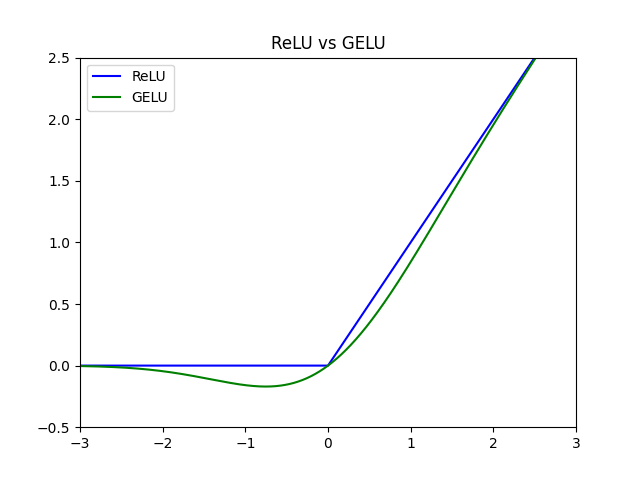
\includegraphics[width=0.9\textwidth]{figures/ml_theory/relu_gelu.png}
		\caption{ReLU and GELU functions}
		\label{fig:relu_gelu}
	\end{subfigure}
	\begin{subfigure}{.5\textwidth}
		\centering
		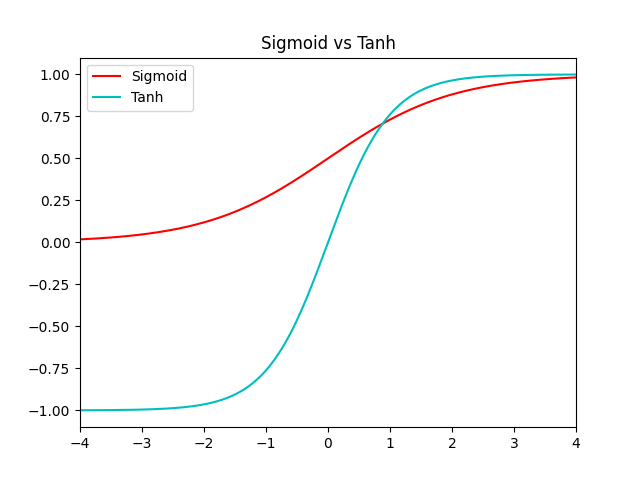
\includegraphics[width=0.9\textwidth]{figures/ml_theory/sigmoid_tanh.png}
		\caption{Sigmoid and Tanh functions}
		\label{fig:sigmoid_tanh}
	\end{subfigure}
	\caption{Activation Functions}
	\label{fig:activation_functions}
\end{figure}

\textbf{ReLU}, defined by
\begin{equation}
\label{eqn:relu_fcn}
\textrm{ReLU}(x) = \max(0, x),
\end{equation}
is a simple function mapping negative values to zero while passing positive values as it is. It is computationally cheap and allows to train deep and complex networks~\cite{glorot_deep_2011}.

\textbf{GELU}, defined by
\begin{equation}
\label{eqn:gelu_fcn}
\textrm{GELU}(x) = x \Phi(x) = \frac{x}{2} \bigg[ 1 + \textrm{erf} \Big( \frac{x}{\sqrt{2}} \Big) \bigg],
\end{equation}
is smoothed version of ReLU function. It is continuous but non-convex and has several advantages \cite{hendrycks_gaussian_2020}. ReLU and GELU are visualized in  \figref{fig:relu_gelu}. 

\subsection{Softmax}

Softmax function is generalization upon sigmoid function and used for multinomial classifications. It is smooth type of $\argmax$ operator. Assume that there is a vector $x \in \mathbb{R}^K$. Softmax assigns probability values to each element, summing up to 1. It is defined as,
\begin{equation}
\label{eqn:softmax_fcn}
\text{softmax}(x) = \frac{\exp(x)}{\sum \exp(x)},
\end{equation}
where exponentiation in denominator applied elementwise and denominator is a scalar.

\subsection{Layer Normalization}

Layer normalization is a layer to overcome instability and divergence during learning~\cite{ba_layer_2016}. 
Given an input $x \in \mathbb{R}^K$, mean and variance statistics are evaluated along the dimensions as  
\begin{equation}
\label{eq:layernorm_statistics}
\begin{split}
\mu = & \frac{1}{K} \sum_{n=1}^{K} x_k \\
\sigma^2 = & \frac{1}{K} \sum_{n=1}^{K} (x_k-\mu)^2
\end{split}.
\end{equation} 
Then, the input is first scaled to have zero mean and unity variance along dimensions. 
The term $\epsilon$ is added to prevent division by zero. 
Optionally, the result is scaled by elementwise multiplication by $\gamma \in \mathbb{R}^K$ and addition by $\beta \in \mathbb{R}^K$ as
\begin{equation}
\label{eqn:layernorm}
\mathrm{LN}(x) = \frac{x-\mu}{\sigma+\epsilon} * \gamma + \beta,
\end{equation}
where $\gamma$ and $\beta$ are learnable parameters. 
